% Options for packages loaded elsewhere
\PassOptionsToPackage{unicode}{hyperref}
\PassOptionsToPackage{hyphens}{url}
\PassOptionsToPackage{dvipsnames,svgnames,x11names}{xcolor}
%
\documentclass[
  letterpaper,
  DIV=11,
  numbers=noendperiod]{scrreprt}

\usepackage{amsmath,amssymb}
\usepackage{iftex}
\ifPDFTeX
  \usepackage[T1]{fontenc}
  \usepackage[utf8]{inputenc}
  \usepackage{textcomp} % provide euro and other symbols
\else % if luatex or xetex
  \usepackage{unicode-math}
  \defaultfontfeatures{Scale=MatchLowercase}
  \defaultfontfeatures[\rmfamily]{Ligatures=TeX,Scale=1}
\fi
\usepackage{lmodern}
\ifPDFTeX\else  
    % xetex/luatex font selection
\fi
% Use upquote if available, for straight quotes in verbatim environments
\IfFileExists{upquote.sty}{\usepackage{upquote}}{}
\IfFileExists{microtype.sty}{% use microtype if available
  \usepackage[]{microtype}
  \UseMicrotypeSet[protrusion]{basicmath} % disable protrusion for tt fonts
}{}
\makeatletter
\@ifundefined{KOMAClassName}{% if non-KOMA class
  \IfFileExists{parskip.sty}{%
    \usepackage{parskip}
  }{% else
    \setlength{\parindent}{0pt}
    \setlength{\parskip}{6pt plus 2pt minus 1pt}}
}{% if KOMA class
  \KOMAoptions{parskip=half}}
\makeatother
\usepackage{xcolor}
\setlength{\emergencystretch}{3em} % prevent overfull lines
\setcounter{secnumdepth}{5}
% Make \paragraph and \subparagraph free-standing
\ifx\paragraph\undefined\else
  \let\oldparagraph\paragraph
  \renewcommand{\paragraph}[1]{\oldparagraph{#1}\mbox{}}
\fi
\ifx\subparagraph\undefined\else
  \let\oldsubparagraph\subparagraph
  \renewcommand{\subparagraph}[1]{\oldsubparagraph{#1}\mbox{}}
\fi

\usepackage{color}
\usepackage{fancyvrb}
\newcommand{\VerbBar}{|}
\newcommand{\VERB}{\Verb[commandchars=\\\{\}]}
\DefineVerbatimEnvironment{Highlighting}{Verbatim}{commandchars=\\\{\}}
% Add ',fontsize=\small' for more characters per line
\usepackage{framed}
\definecolor{shadecolor}{RGB}{241,243,245}
\newenvironment{Shaded}{\begin{snugshade}}{\end{snugshade}}
\newcommand{\AlertTok}[1]{\textcolor[rgb]{0.68,0.00,0.00}{#1}}
\newcommand{\AnnotationTok}[1]{\textcolor[rgb]{0.37,0.37,0.37}{#1}}
\newcommand{\AttributeTok}[1]{\textcolor[rgb]{0.40,0.45,0.13}{#1}}
\newcommand{\BaseNTok}[1]{\textcolor[rgb]{0.68,0.00,0.00}{#1}}
\newcommand{\BuiltInTok}[1]{\textcolor[rgb]{0.00,0.23,0.31}{#1}}
\newcommand{\CharTok}[1]{\textcolor[rgb]{0.13,0.47,0.30}{#1}}
\newcommand{\CommentTok}[1]{\textcolor[rgb]{0.37,0.37,0.37}{#1}}
\newcommand{\CommentVarTok}[1]{\textcolor[rgb]{0.37,0.37,0.37}{\textit{#1}}}
\newcommand{\ConstantTok}[1]{\textcolor[rgb]{0.56,0.35,0.01}{#1}}
\newcommand{\ControlFlowTok}[1]{\textcolor[rgb]{0.00,0.23,0.31}{#1}}
\newcommand{\DataTypeTok}[1]{\textcolor[rgb]{0.68,0.00,0.00}{#1}}
\newcommand{\DecValTok}[1]{\textcolor[rgb]{0.68,0.00,0.00}{#1}}
\newcommand{\DocumentationTok}[1]{\textcolor[rgb]{0.37,0.37,0.37}{\textit{#1}}}
\newcommand{\ErrorTok}[1]{\textcolor[rgb]{0.68,0.00,0.00}{#1}}
\newcommand{\ExtensionTok}[1]{\textcolor[rgb]{0.00,0.23,0.31}{#1}}
\newcommand{\FloatTok}[1]{\textcolor[rgb]{0.68,0.00,0.00}{#1}}
\newcommand{\FunctionTok}[1]{\textcolor[rgb]{0.28,0.35,0.67}{#1}}
\newcommand{\ImportTok}[1]{\textcolor[rgb]{0.00,0.46,0.62}{#1}}
\newcommand{\InformationTok}[1]{\textcolor[rgb]{0.37,0.37,0.37}{#1}}
\newcommand{\KeywordTok}[1]{\textcolor[rgb]{0.00,0.23,0.31}{#1}}
\newcommand{\NormalTok}[1]{\textcolor[rgb]{0.00,0.23,0.31}{#1}}
\newcommand{\OperatorTok}[1]{\textcolor[rgb]{0.37,0.37,0.37}{#1}}
\newcommand{\OtherTok}[1]{\textcolor[rgb]{0.00,0.23,0.31}{#1}}
\newcommand{\PreprocessorTok}[1]{\textcolor[rgb]{0.68,0.00,0.00}{#1}}
\newcommand{\RegionMarkerTok}[1]{\textcolor[rgb]{0.00,0.23,0.31}{#1}}
\newcommand{\SpecialCharTok}[1]{\textcolor[rgb]{0.37,0.37,0.37}{#1}}
\newcommand{\SpecialStringTok}[1]{\textcolor[rgb]{0.13,0.47,0.30}{#1}}
\newcommand{\StringTok}[1]{\textcolor[rgb]{0.13,0.47,0.30}{#1}}
\newcommand{\VariableTok}[1]{\textcolor[rgb]{0.07,0.07,0.07}{#1}}
\newcommand{\VerbatimStringTok}[1]{\textcolor[rgb]{0.13,0.47,0.30}{#1}}
\newcommand{\WarningTok}[1]{\textcolor[rgb]{0.37,0.37,0.37}{\textit{#1}}}

\providecommand{\tightlist}{%
  \setlength{\itemsep}{0pt}\setlength{\parskip}{0pt}}\usepackage{longtable,booktabs,array}
\usepackage{calc} % for calculating minipage widths
% Correct order of tables after \paragraph or \subparagraph
\usepackage{etoolbox}
\makeatletter
\patchcmd\longtable{\par}{\if@noskipsec\mbox{}\fi\par}{}{}
\makeatother
% Allow footnotes in longtable head/foot
\IfFileExists{footnotehyper.sty}{\usepackage{footnotehyper}}{\usepackage{footnote}}
\makesavenoteenv{longtable}
\usepackage{graphicx}
\makeatletter
\def\maxwidth{\ifdim\Gin@nat@width>\linewidth\linewidth\else\Gin@nat@width\fi}
\def\maxheight{\ifdim\Gin@nat@height>\textheight\textheight\else\Gin@nat@height\fi}
\makeatother
% Scale images if necessary, so that they will not overflow the page
% margins by default, and it is still possible to overwrite the defaults
% using explicit options in \includegraphics[width, height, ...]{}
\setkeys{Gin}{width=\maxwidth,height=\maxheight,keepaspectratio}
% Set default figure placement to htbp
\makeatletter
\def\fps@figure{htbp}
\makeatother
\newlength{\cslhangindent}
\setlength{\cslhangindent}{1.5em}
\newlength{\csllabelwidth}
\setlength{\csllabelwidth}{3em}
\newlength{\cslentryspacingunit} % times entry-spacing
\setlength{\cslentryspacingunit}{\parskip}
\newenvironment{CSLReferences}[2] % #1 hanging-ident, #2 entry spacing
 {% don't indent paragraphs
  \setlength{\parindent}{0pt}
  % turn on hanging indent if param 1 is 1
  \ifodd #1
  \let\oldpar\par
  \def\par{\hangindent=\cslhangindent\oldpar}
  \fi
  % set entry spacing
  \setlength{\parskip}{#2\cslentryspacingunit}
 }%
 {}
\usepackage{calc}
\newcommand{\CSLBlock}[1]{#1\hfill\break}
\newcommand{\CSLLeftMargin}[1]{\parbox[t]{\csllabelwidth}{#1}}
\newcommand{\CSLRightInline}[1]{\parbox[t]{\linewidth - \csllabelwidth}{#1}\break}
\newcommand{\CSLIndent}[1]{\hspace{\cslhangindent}#1}

\KOMAoption{captions}{tableheading}
\makeatletter
\makeatother
\makeatletter
\@ifpackageloaded{bookmark}{}{\usepackage{bookmark}}
\makeatother
\makeatletter
\@ifpackageloaded{caption}{}{\usepackage{caption}}
\AtBeginDocument{%
\ifdefined\contentsname
  \renewcommand*\contentsname{Table of contents}
\else
  \newcommand\contentsname{Table of contents}
\fi
\ifdefined\listfigurename
  \renewcommand*\listfigurename{List of Figures}
\else
  \newcommand\listfigurename{List of Figures}
\fi
\ifdefined\listtablename
  \renewcommand*\listtablename{List of Tables}
\else
  \newcommand\listtablename{List of Tables}
\fi
\ifdefined\figurename
  \renewcommand*\figurename{Figure}
\else
  \newcommand\figurename{Figure}
\fi
\ifdefined\tablename
  \renewcommand*\tablename{Table}
\else
  \newcommand\tablename{Table}
\fi
}
\@ifpackageloaded{float}{}{\usepackage{float}}
\floatstyle{ruled}
\@ifundefined{c@chapter}{\newfloat{codelisting}{h}{lop}}{\newfloat{codelisting}{h}{lop}[chapter]}
\floatname{codelisting}{Listing}
\newcommand*\listoflistings{\listof{codelisting}{List of Listings}}
\makeatother
\makeatletter
\@ifpackageloaded{caption}{}{\usepackage{caption}}
\@ifpackageloaded{subcaption}{}{\usepackage{subcaption}}
\makeatother
\makeatletter
\@ifpackageloaded{tcolorbox}{}{\usepackage[skins,breakable]{tcolorbox}}
\makeatother
\makeatletter
\@ifundefined{shadecolor}{\definecolor{shadecolor}{rgb}{.97, .97, .97}}
\makeatother
\makeatletter
\makeatother
\makeatletter
\makeatother
\ifLuaTeX
  \usepackage{selnolig}  % disable illegal ligatures
\fi
\IfFileExists{bookmark.sty}{\usepackage{bookmark}}{\usepackage{hyperref}}
\IfFileExists{xurl.sty}{\usepackage{xurl}}{} % add URL line breaks if available
\urlstyle{same} % disable monospaced font for URLs
\hypersetup{
  pdftitle={Finite Mathematics},
  pdfauthor={Joash Geteregechi},
  colorlinks=true,
  linkcolor={blue},
  filecolor={Maroon},
  citecolor={Blue},
  urlcolor={Blue},
  pdfcreator={LaTeX via pandoc}}

\title{Finite Mathematics}
\author{Joash Geteregechi}
\date{2023-08-04}

\begin{document}
\maketitle
\ifdefined\Shaded\renewenvironment{Shaded}{\begin{tcolorbox}[enhanced, breakable, boxrule=0pt, interior hidden, sharp corners, borderline west={3pt}{0pt}{shadecolor}, frame hidden]}{\end{tcolorbox}}\fi

\renewcommand*\contentsname{Table of contents}
{
\hypersetup{linkcolor=}
\setcounter{tocdepth}{2}
\tableofcontents
}
\bookmarksetup{startatroot}

\hypertarget{preface}{%
\chapter*{Preface}\label{preface}}
\addcontentsline{toc}{chapter}{Preface}

\markboth{Preface}{Preface}

This was made using Quarto.

To learn more about Quarto books visit
\url{https://quarto.org/docs/books}.

\bookmarksetup{startatroot}

\hypertarget{introduction}{%
\chapter{Introduction}\label{introduction}}

This is a book created from markdown and executable code.

See Knuth (1984) for additional discussion of literate programming.

\part{Linear Functions}

\hypertarget{intro-to-linear-functions}{%
\chapter{Intro to Linear Functions}\label{intro-to-linear-functions}}

\hypertarget{definitions-and-notation-for-linear-functions}{%
\section{Definitions and Notation for Linear
Functions}\label{definitions-and-notation-for-linear-functions}}

As you hop into a taxicab in Allentown, the meter will immediately read
\$3.30; this is the ``drop'' charge made when the taximeter is
activated. After that initial fee, the taximeter will add \$2.40 for
each mile the taxi drives. In this scenario, the total taxi fare depends
upon the number of miles ridden in the taxi, and we can ask whether it
is possible to model this type of scenario with a function. Using
descriptive variables, we choose \(m\) for miles and \(C\) for Cost in
dollars as a function of miles: \(C(m)\).

Here, \(C(0)\) means the cost for travelling 0 miles (assuming you have
entered the taxi). This cost is \(\$3.3\). We can write this
mathematically as

\begin{Shaded}
\begin{Highlighting}[]
\DataTypeTok{C}\ErrorTok{(}\DataTypeTok{0}\ErrorTok{)}\OperatorTok{=}\FloatTok{3.3}
\end{Highlighting}
\end{Shaded}

Similarly, \(C(2)\) is the cost of travelling 2 miles and can be
computed as

\begin{Shaded}
\begin{Highlighting}[]
\DataTypeTok{C}\ErrorTok{(}\DataTypeTok{2}\ErrorTok{)} \OperatorTok{=} \FloatTok{3.3} \ErrorTok{+} \ErrorTok{(}\DataTypeTok{2}\KeywordTok{.}\DataTypeTok{4} \DataTypeTok{x} \DataTypeTok{2}\ErrorTok{)} \OperatorTok{=} \FloatTok{8.1}
\end{Highlighting}
\end{Shaded}

Here, we take the base charge of \(\$3.3\) and add it to the charge for
riding 2 miles to get a grand total of 8.1.

In general, if we travel \(m\) miles, we can compute the cost as

\begin{Shaded}
\begin{Highlighting}[]
\DataTypeTok{C}\ErrorTok{(}\DataTypeTok{m}\ErrorTok{)}\OperatorTok{=}\FloatTok{3.3} \ErrorTok{+} \DataTypeTok{2}\KeywordTok{.}\DataTypeTok{4m}
\end{Highlighting}
\end{Shaded}

It is often useful to think carefully about the units of each component
and how they relate. The expression below shows how this plays out in
our taxi context:

\[C(m)=3.3 \hspace{.1in} dollars + 2.4 \hspace{.08in} \frac{dollars}{mile} \times m\hspace{.1in} miles\]

When dollars per mile are multiplied by a number of miles, the result is
a number of dollars, matching the units on the 3.30, and matching the
desired units for the C function. This means the units for the output,
C(m), will be dollars.

We call a relationship such as this, a \textbf{\emph{Function}} of
\(m\). This function takes \(m\) (the miles traveled) as the
\textbf{\emph{Input}} and produces \(C(m)\) (the cost of travelling
\(m\) miles) as the \textbf{\emph{Output}}. As you will learn shortly,
this is an example of a \textbf{\emph{Linear Function}}. There are other
types of functions (e.g., exponential, quadratic, etc.). In this course,
the main focus is on linear functions. We will learn how to model real
life situations and find their solutions by leveraging the ideas learned
under linear functions.

There are two parts to the function, the first part (3.3) represents the
FIXED charge while the VARIABLE part, \(2.4m\) which represents the
charge for m miles. The cost of a ride, \(C(m)\) will vary as the number
of miles, \(m\) varies. Furthermore, this cost varies by a factor of 2.4
which means that for every additional mile you ride, you will pay
\(\$ 2.4\) more. We call the value \(2.4\) a \textbf{\emph{Rate of
Change}} for the function \(C(m)\). Since this rate of change stays the
same over any interval, we say that the rate is
\textbf{\emph{Constant}}.

\hypertarget{function-representations}{%
\section{Function Representations}\label{function-representations}}

In the above section, we described the taxi cost function using words
and represented it using a formula. Functions can also be represented
using tables and graphs.

Consider the table below:

\textbf{\emph{Have table here}}

We can also represent the function using a graph as shown below:

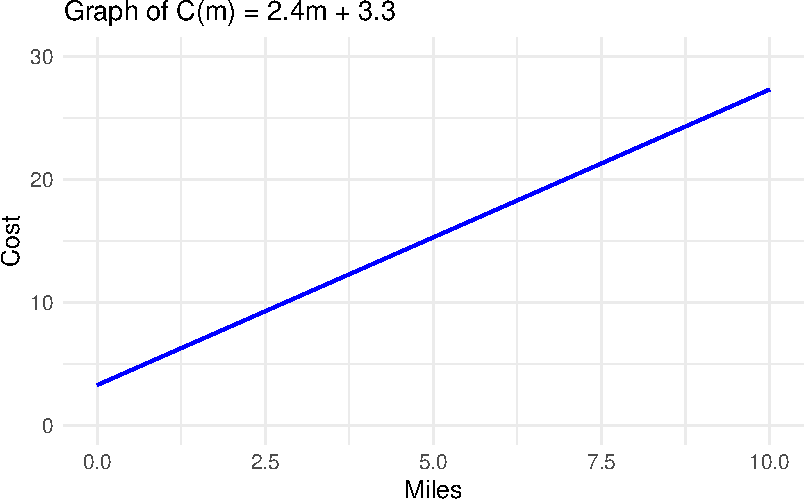
\includegraphics{Intro_LF_files/figure-pdf/unnamed-chunk-1-1.pdf}

In the graph, we place the miles on the horizontal axis and the cost on
the vertical axis axis. Since the cost is dependent on the miles
traveled, we call it a \textbf{\emph{Dependent Variable}}. Similarly, we
call the miles, an \textbf{\emph{Independent Variable}}.

If you ride 0 miles, the cost is \$3.30, giving the point (0, 3.30) on
the graph. We call this, the vertical or C(m)-intercept (or y-intercept
in a general graph using x and y). In many applications, the y-intercept
often means the initial value (e.g., cost) when the x value (in this
case miles) is zero.

We call the above function, a \textbf{\emph{Linear Function}} because
its graph produces a straight line. In general, linear functions take
the form \(f(x)=mx+b\) where \(m\) is the \textbf{\emph{Slope}} (or rate
of change) and \(b\) is the y-intercept. Note that \(b\) and/or \(m\)
can take any values including zero.

By convention, we place the output values on the vertical (\(y\)) axis
and so, \(y\) can be used in place of \(f(x)\). Hence, we can rewrite
the above function as an equation: \[y=mx+b\]

\hypertarget{increasing-and-decreasing-functions}{%
\section{Increasing and Decreasing
Functions}\label{increasing-and-decreasing-functions}}

Notice in the above example that as you increase the number of miles,
the cost of the ride goes up. This is because the rate of change (m) is
positive.

Since as you increase the input value, the output value increases, we
say that the function \(C(m)\) is an increasing function. As can be seen
on the graph, the line is rising from left to right. This is because the
rate of change value is positive.

Generally, a linear function is said to be \textbf{\emph{increasing}} if
the slope \(m\) is positive and

\textbf{\emph{decreasing}} if it is negative.

\textbf{EXERCISE}

\begin{Shaded}
\begin{Highlighting}[]
\DataTypeTok{1}\KeywordTok{.} \DataTypeTok{Create} \DataTypeTok{a} \DataTypeTok{real{-}life} \DataTypeTok{scenario} \DataTypeTok{that} \DataTypeTok{can} \DataTypeTok{be} \DataTypeTok{modelled} \DataTypeTok{by} \DataTypeTok{a} \DataTypeTok{decreasing} \DataTypeTok{linear} \DataTypeTok{function}
\DataTypeTok{2}\KeywordTok{.} \DataTypeTok{Write} \DataTypeTok{the} \DataTypeTok{formula} \DataTypeTok{for} \DataTypeTok{the} \DataTypeTok{function} \DataTypeTok{and} \DataTypeTok{graph} \DataTypeTok{it}\KeywordTok{.}
\DataTypeTok{3}\KeywordTok{.} \DataTypeTok{What} \DataTypeTok{would} \DataTypeTok{the} \DataTypeTok{graph} \DataTypeTok{of} \DataTypeTok{the} \DataTypeTok{function}\ErrorTok{,} \DataTypeTok{f}\ErrorTok{(}\DataTypeTok{x}\ErrorTok{)}\OperatorTok{=} \DecValTok{0}\DataTypeTok{x}\ErrorTok{+}\DataTypeTok{5} \DataTypeTok{look} \DataTypeTok{like}\ErrorTok{?} \DataTypeTok{Notice} \DataTypeTok{here} \DataTypeTok{m} \OperatorTok{=} \DecValTok{0}\KeywordTok{.} 
\end{Highlighting}
\end{Shaded}

\hypertarget{rate-of-change}{%
\chapter{Rate of Change}\label{rate-of-change}}

\hypertarget{calculating-rate-of-change}{%
\section{Calculating Rate of Change}\label{calculating-rate-of-change}}

The rate of change (ROC) is perhaps the most important component of any
linear function. As we have seen, it can tell you whether the function
is increasing or decreasing and can be used to create a linear model for
a given real life situation. The question that arises is, ``how can we
compute the rate of change from given data?''. In the earlier taxi
example, suppose, we did not know the rate of change but knew the cots
of riding 4 miles and 7 miles. How can we use this information together
with the fact that the function is linear to find the rate of change?

In the following examples we explore ways of finding the rate of change
and how to use it to create the linear function/model for given
real-life situations.

\textbf{Example 1}

The population of a city can be modeled using a linear function. In
2002, the population was 23,400 and in 2006, it was 27,800.

\begin{enumerate}
\def\labelenumi{\alph{enumi})}
\item
  Find the rate of change of the population for this city.
\item
  Write down the formula of the linear function for the scenario.
\item
  Assuming the model (function) holds true until 2024, what would be the
  population of the town in 2024?
\end{enumerate}

\textbf{\emph{Solution}}

\begin{enumerate}
\def\labelenumi{\alph{enumi})}
\tightlist
\item
  Since we are told that the population grows linearly, we know that the
  growth between 2002 and 2003 is the same as the growth between 2003
  and 2004, etc. Thus, to find the rate of change (i.e., population
  growth per year), we can divide the population change between 2002 and
  2006 by the number of years as shown:
\end{enumerate}

\begin{align} 
Rate\hspace{.04in} of\hspace{.04in} change &=  \frac{pop. \hspace{.04in} in \hspace{.04in} 2006 \hspace{.04in}- pop. \hspace{.04in} in \hspace{.04in} 2002}{2006-2002}\\&= 1100\hspace{.04in} people\hspace{.04in} per \hspace{.04in} year
\end{align}

\begin{enumerate}
\def\labelenumi{\alph{enumi})}
\setcounter{enumi}{1}
\tightlist
\item
  If we use 2002 as the base year(i.e., t=0), then the constant value in
  the function is 23,400. Next, since we have the rate of change, all we
  need is to write the function in the form \(f(x)=mx+b\) where \(m\) is
  the rate of change and \(b\) is the constant or initial value, and t
  is time in years.
\end{enumerate}

\[f(t) = 1100t+23,400\]

\begin{enumerate}
\def\labelenumi{\alph{enumi})}
\setcounter{enumi}{2}
\tightlist
\item
  For 2024, \(t=22\) years. Thus,
\end{enumerate}

\begin{align}
f(22) &= 1100\times22+23,400\\&=47,600
\end{align}

\textbf{Example 2}

The summit of Africa's largest peak, Mt. Kilimanjaro, has two main ice
fields and a glacier at its peak. Geologists measured the ice cover in
the year 2000 (\(t = 0\)) to be approximately \(1951\hspace{.05in}m^2\);
in the year 2007, the ice cover measured \(1555 \hspace{.05in}m^2\).

\begin{enumerate}
\def\labelenumi{\alph{enumi})}
\item
  Suppose that the amount of ice cover at the peak of Mt. Kilimanjaro is
  changing at a constant average rate from year to year. Find a linear
  model, \(A=f(t)\) whose output is the area, A, in square meters in
  year \(t\) (where is the number of years after 2000).
\item
  What do the slope and \(A\)-intercept mean in the model you found in
  (a)? In particular, what are the units on the slope?
\end{enumerate}

\begin{enumerate}
\def\labelenumi{\Alph{enumi})}
\setcounter{enumi}{2}
\tightlist
\item
  Compute \(f(17)\). What does this quantity measure? Write a complete
  sentence to explain.
\end{enumerate}

\begin{enumerate}
\def\labelenumi{\alph{enumi})}
\setcounter{enumi}{3}
\tightlist
\item
  If the model holds further into the future, when do we predict the ice
  cover will vanish?
\end{enumerate}

\textbf{\emph{Solution}}

\begin{enumerate}
\def\labelenumi{\alph{enumi})}
\tightlist
\item
  We begin by finding the rate of change. Since we know that the rate of
  change is constant year after year, we can divide the change between
  2007 and 2000 by 7 to get the rate of change. \begin{align}
  Rate\hspace{.04in} of\hspace{.04in} change &=  \frac{Coverage \hspace{.04in} in \hspace{.04in} 2007 \hspace{.04in}- Coverage \hspace{.04in} in \hspace{.04in} 2000}{2007-2000}\\
  &= - 56.57\hspace{.04in} m^2\hspace{.04in} per \hspace{.04in} year
  \end{align} The general format of a linear function is \(A(t)=mt+b\)
  where \(m\) is the rate of change and \(b\) is the \(A(t)\)-intercept
  (or the value of \(A(0)\) which we know is 1951). Thus, the function
  is,
\end{enumerate}

\[A(t)=-56.57t + 1951\]

\begin{enumerate}
\def\labelenumi{\alph{enumi})}
\setcounter{enumi}{1}
\item
  The slope means that the ice for every additional year, the ice
  coverage decreases by \(56.57 m^2\). The units are square meters per
  year (\(m^2/year\)). The y intercept means that the initial coverage
  at year zero (when the measurement was first taken) is \(1951 m^2\).
\item
  \(f(17)=(-55.57\times17)+1951=1006.31\); This means that there were
  \(1006.31 mi^2\) of ice coverage on Mt. Kilimanjaro by 2017 (i.e., 17
  years after 2000).
\item
  Remember that \(A(t)\) is the function that gives the ice cover after
  to years. Therefore, if the ice cover is zero, it means \(A(t)=0\). We
  compute \(t\) by solving the equation \(-56.57t + 1951=0\) for t.
\end{enumerate}

\begin{align}
  -56.57t + 1951&=0\\
  -56.57t&=-1951\\
  t&=\frac{-1951}{-56.57}\\
  t&=34.49 \hspace{0.04in} years
  \end{align}

\hypertarget{a-formula-for-roc}{%
\subsection{A Formula For ROC}\label{a-formula-for-roc}}

From the foregoing examples, it should be readily clear that, on any
interval \((x_1,x_2)\) where \(x_1\neq x_2\),

\begin{align}
  Rate \hspace{0.04in}of\hspace{0.04in} Change                         
  &=\frac{Change\hspace{0.04in}in\hspace{0.04in}Output}{Change \hspace{0.04in}         
  in\hspace{0.04in}Input}\\
  &=\frac{f(x_2)-f(x_1)}{x_2 - x_1}
  \end{align}

\textbf{Example 3}

If \(f(x)\) is a linear function, \(f(3)=−2\), and \(f(8)=1\), find an
equation/formula for the function.

\textbf{\emph{Solution}}

In this problem, we are looking at the input interval between 3 and 8.
Thus, \(x_1=3\) and \(x_2=8\). To find the ROC for \(f(x)\) we proceed
as follows:

\begin{align}
ROC &= \frac{f(x_2)-f(x_1)}{x_2 - x_1}\\
&= \frac{f(3)-f(1)}{8 - 3}\\
&= \frac{1-(-2)}{5}\\
&=\frac{3}{5}
\end{align} Next, the general form of the linear function is
\(f(x)=mx+b\), where \(m\) is the ROC (aka slope. So, we can write,
\(f(x)=\frac{3}{5}x+b\). To find \(b\), we can use one of the known
values of \(f(x)\), such as \(f(8)\) and solve for \(b\) as follows:

\begin{align}
f(8)&=\frac{3}{5}\times (8)+b\\
1&=\frac{24}{5}+b\\
b&=1-\frac{24}{5}\\
&=-\frac{19}{5}
\end{align}

So, the equation becomes,

\[f(x)=\frac{3}{5}x-\frac{19}{5}\]

\hypertarget{point-slope-equation-format}{%
\section{Point-Slope Equation
Format}\label{point-slope-equation-format}}

The equation \(y=mx+b\) is called the slope-intercept form of a linear
function (equation). In cases where you only know one of the points, say
\((x_1,y_1)\) and the slope \(m\) you can express the equation of the
line as follows:

\[y-y_1=m(x-x_1)\] Where, \((x_1,y_1)\) is the KNOWN point.

After this, you can then rearrange the equation into the slope-intercept
format. You just need to be careful with your algebraic manipulation
when doing this. See example below:

\textbf{Example 4}

A new house was sold for \$296000 8 years after it was purchased. The
original owners calculated that the house appreciated \$2,500 per year
while they owned it. Find a linear function that describes the above
situation if \(x\) is the number of years since the building was
purchased.

\textbf{\emph{Solution}}

Let \(x\) be the number of years and \(C(x)\) be the cost of the house
after \(x\) years.

Note that, we do not know the initial price (i.e., \(b\)) but we know
the \(ROC\) in cost to be 2,500 \$ per year (i.e., a linear function).
We also know the cost after 8 years (i.e, we know one point
\((8, 296,000)\)).

We can use this information and the concept of slope-point format to
write the equation of the line as follows:

\begin{align}
y-y_1&=m(x-x_1)\\
y-296,000&=2500(x-8)\\
y-296,000&=2500x-20,000\\
y&=2500x-20000+296,000\\
y&=2500x+276,000
\end{align}

Note that in the above equation, \(y=C(x)\). So we are done. As a bonus,
we know the cost of the house was \$276,000 eight years ago.

\hypertarget{applications}{%
\chapter{Applications}\label{applications}}

\hypertarget{equation-of-a-line}{%
\section{Equation of a Line}\label{equation-of-a-line}}

\hypertarget{parallel-intersecting-lines}{%
\section{Parallel Intersecting
Lines}\label{parallel-intersecting-lines}}

\hypertarget{graphin-linear-functions}{%
\section{Graphin Linear Functions}\label{graphin-linear-functions}}

\hypertarget{systems-of-equations}{%
\section{Systems of Equations}\label{systems-of-equations}}

\part{Linear Programming}

\hypertarget{intro-to-linear-programming}{%
\chapter{Intro to Linear
Programming}\label{intro-to-linear-programming}}

\hypertarget{geometric-method}{%
\chapter{Geometric Method}\label{geometric-method}}

\hypertarget{introduction-to-linear-programming}{%
\section{Introduction to linear
Programming}\label{introduction-to-linear-programming}}

Managers are often called upon to make complicated decisions. For
example, production managers often make decisions on what products to
manufacture and in what quantities. In making such decisions, the
manager must consider the available resources and how to utilize them
for maximum profit. Note that resources are not limited to raw
materials. They can include labor (human hours), farmland, machinery,
etc. Resources, in general, are always limited and management must
decide how to allocate them in order to get the maximum possible profit.

Linear programming (LP) is one of the most important methods used in
management science to solve problems of the kind describe above. LP
involves maximizing or minimizing a quantity, usually profit or cost,
under some given constraints.

\hypertarget{mixture-problems-charts}{%
\section{Mixture Problems \& Charts}\label{mixture-problems-charts}}

A mixture problem is a problem which includes combining limited
resources to manufacture products that will generate maximum profit for
the company.

These problems are common because most products that we use involve
combining multiple resources in their production. Although there are
other considerations in making production decisions, availability of
resources is on of the most important constraints.

An \textbf{\emph{optimal production policy (OPP)}} is a policy that,

\begin{Shaded}
\begin{Highlighting}[]
\ErrorTok{(}\DataTypeTok{i}\ErrorTok{)} \DataTypeTok{does} \DataTypeTok{not} \DataTypeTok{violate} \DataTypeTok{the} \DataTypeTok{constraints} \DataTypeTok{under} \DataTypeTok{which} \DataTypeTok{the} \DataTypeTok{comany} \DataTypeTok{operates} \DataTypeTok{and}\ErrorTok{,}
\ErrorTok{(}\DataTypeTok{ii}\ErrorTok{)} \DataTypeTok{gives} \DataTypeTok{maximum} \DataTypeTok{profit}\KeywordTok{.}
\end{Highlighting}
\end{Shaded}

\textbf{Example 1}

A toy manufacturer can manufacture only skateboards and, only dolls, or
some kind of skateboards and dolls. Skateboards require 5 units of
plastic and can be sold for a profit of \$ 1, while dolls require 2
units of plastic and can be sold for \$0.55 profit. Only 60 units of
plastic are available.

\begin{enumerate}
\def\labelenumi{(\alph{enumi})}
\tightlist
\item
  Make a mixture chart to model this situation.
\item
  What numbers of skateboards and/or dolls should the company make to
  maximize profit?
\end{enumerate}

Before we solve this problem, note that it is a mixture problem because:

\begin{itemize}
\item
  Definite resources are available in limited quantities. The resource
  here is container units of plastic.
\item
  Definite products can be made by combining (mixing) the resources. The
  products here are skateboards and dolls.
\end{itemize}

\textbf{\emph{Solution}}

\begin{enumerate}
\def\labelenumi{\alph{enumi})}
\tightlist
\item
  A mixture is a simple table that shows the resources, products, and
  profit. The chart displays the ``verbal'' information into a format
  that makes it easier to convert the problem to mathematical form
  (equations) that we can then solve it. The rows of the mixture chart
  contain the products while the columns contain the resources and the
  profit margin. See below:
\end{enumerate}

\begin{longtable}[]{@{}
  >{\centering\arraybackslash}p{(\columnwidth - 4\tabcolsep) * \real{0.2778}}
  >{\centering\arraybackslash}p{(\columnwidth - 4\tabcolsep) * \real{0.5139}}
  >{\raggedleft\arraybackslash}p{(\columnwidth - 4\tabcolsep) * \real{0.2083}}@{}}
\caption{\textbf{Mixture Chart for dolls and skateboards
problem}}\tabularnewline
\toprule\noalign{}
\begin{minipage}[b]{\linewidth}\centering
Products
\end{minipage} & \begin{minipage}[b]{\linewidth}\centering
Resource(s): Containers of plastic: 60
\end{minipage} & \begin{minipage}[b]{\linewidth}\raggedleft
Profit
\end{minipage} \\
\midrule\noalign{}
\endfirsthead
\toprule\noalign{}
\begin{minipage}[b]{\linewidth}\centering
Products
\end{minipage} & \begin{minipage}[b]{\linewidth}\centering
Resource(s): Containers of plastic: 60
\end{minipage} & \begin{minipage}[b]{\linewidth}\raggedleft
Profit
\end{minipage} \\
\midrule\noalign{}
\endhead
\bottomrule\noalign{}
\endlastfoot
Skateboard (x units) & 5 & \$ 1.00 \\
Dolls(y units) & 2 & \$ 0.55 \\
\end{longtable}

\begin{enumerate}
\def\labelenumi{\alph{enumi})}
\setcounter{enumi}{1}
\item
  To solve this problem, we will have to follow a series of steps which
  include:

  \begin{itemize}
  \tightlist
  \item
    Translating the problem into a mathematical form,
  \item
    Identifying a set of possible solutions (feasible region) and,
  \item
    Identifying a solution that would give us maximum profit, i.e., the
    optimal b production policy.
  \end{itemize}
\end{enumerate}

There are several methods solving linear programming problems. We will
start with the geometric method, then look at the simplex method, and
finally MS excel. We will talk about the pros and cons of each method.

\hypertarget{the-geometric-method}{%
\section{The Geometric Method}\label{the-geometric-method}}

The geometric method of solving linear programming problems involves
creating a graph to visualize the \textbf{feasible region} (the set of
likely solutions) and then identifying a solution from the feasible
region.

\begin{Shaded}
\begin{Highlighting}[]
\DataTypeTok{A} \DataTypeTok{feasible} \DataTypeTok{set} \ErrorTok{(}\DataTypeTok{region}\ErrorTok{)} \DataTypeTok{for} \DataTypeTok{an} \DataTypeTok{LP} \DataTypeTok{problem} \DataTypeTok{is} \DataTypeTok{the} \DataTypeTok{collection} \DataTypeTok{of} \DataTypeTok{all} \DataTypeTok{physical}
\DataTypeTok{possible} \DataTypeTok{solution} \DataTypeTok{choices} \DataTypeTok{that} \DataTypeTok{can} \DataTypeTok{be} \DataTypeTok{made}\KeywordTok{.} 
\end{Highlighting}
\end{Shaded}

\hypertarget{convering-mixture-chart-into-mathematical-form}{%
\subsection{Convering Mixture Chart into Mathematical
Form}\label{convering-mixture-chart-into-mathematical-form}}

First, we know that the we cannot manufacture negative number of objects
(skateboards of dolls). So, negative numbers are not permitted in this
context. Note however, that 0 is a possible number. Thus, we have two
inequalities;

\[x \ge 0 \hspace{.04in} \text{and} \hspace{.04in} y \ge 0\]

The symbol \(>\) means grater than while \(\ge\) means greater than or
equal to.

We call the above two inequalities \textbf{\emph{minimum constraints}}
because they tell us the minimum that we can have for each object.

Since we have a limited supply of resources (in this case 60 units of
plastic) we must also have inequalities for \textbf{\emph{resource
constraints}}. Since we need 5 units of plastic to manufacture ONE
skateboard, we will need \(5x\) units to manufacture x units of
skateboards. Similarly, we will need \(2y\) units of plastic to
manufacture y dolls. In total, we need \(5x+2y\) units of plastic to
manufacture the dolls and skateboard. This value must not exceed 60.
Thus, we have the inequality,

\[5x+2y\le60\]

Notice that this time, we use the symbol for less than or equal to.

In this problem, we only have 3 inequalities but in a realistic problem,
there would be hundreds or even thousands of them.

The last step in formulating the mathematical model is to make the
\textbf{objective function}. This is the the function that connects the
profit to the resources. Since we know that each skateboard results in
\$1.00 profit, we know that x dolls will result in a profit of \(\$1x\)
and y dolls will result in a profit of \(\$0.55x\). We do not know what
the profit is but we know it is a function of both dolls and
skateboards. We can denote the profit as \(P\). So, we have the
equation,

\[P=1x+0.55y\] Notice that the objective function is an
\textbf{equation} (not inequality) that gives a \textbf{specific} amount
of profit as we vary the number of skateboards and dolls. In other
words, \(P\) changes as we change \(x\) and \(y\). So we can determine
the value of \(x\) and\(y\) that would produce maximum \(P\).

\hypertarget{representing-the-feasible-region}{%
\subsection{Representing the Feasible
Region}\label{representing-the-feasible-region}}

After creating the inequalities from the mixture chart, we can draw a
helpful picture to help us visualize the feasible region geometrically.
Graphs are the most commonly used tools for visualizing the feasible
region.

Notice that all the three inequalities (i.e., the minimum and resource
constraints) are linear in the sense that when you graph them (assuming
an equal sign) you will get a straight line. To take care of the fact
that the inequalities admit a broad range of values, we,

\begin{enumerate}
\def\labelenumi{\alph{enumi})}
\tightlist
\item
  Use a dotted line if the inequality is strictly less \((<)\) or
  greater \((>)\) and shade the region representing the constraints. For
  example, \(x>0\), represents the \(y-axis\) so we draw a dotted line
  there and shade the right side of the line (i.e., values for which
  \(x>0\).
\item
  Use a bold line if the inequality allows equality (e.g., \(x\ge0\)).
  In this case, we would draw the same line as (a) above but without
  dotting it (i.e, a continuous line.
\end{enumerate}

Below is a graph of the feasible region for our problem above

\begin{figure}

{\centering 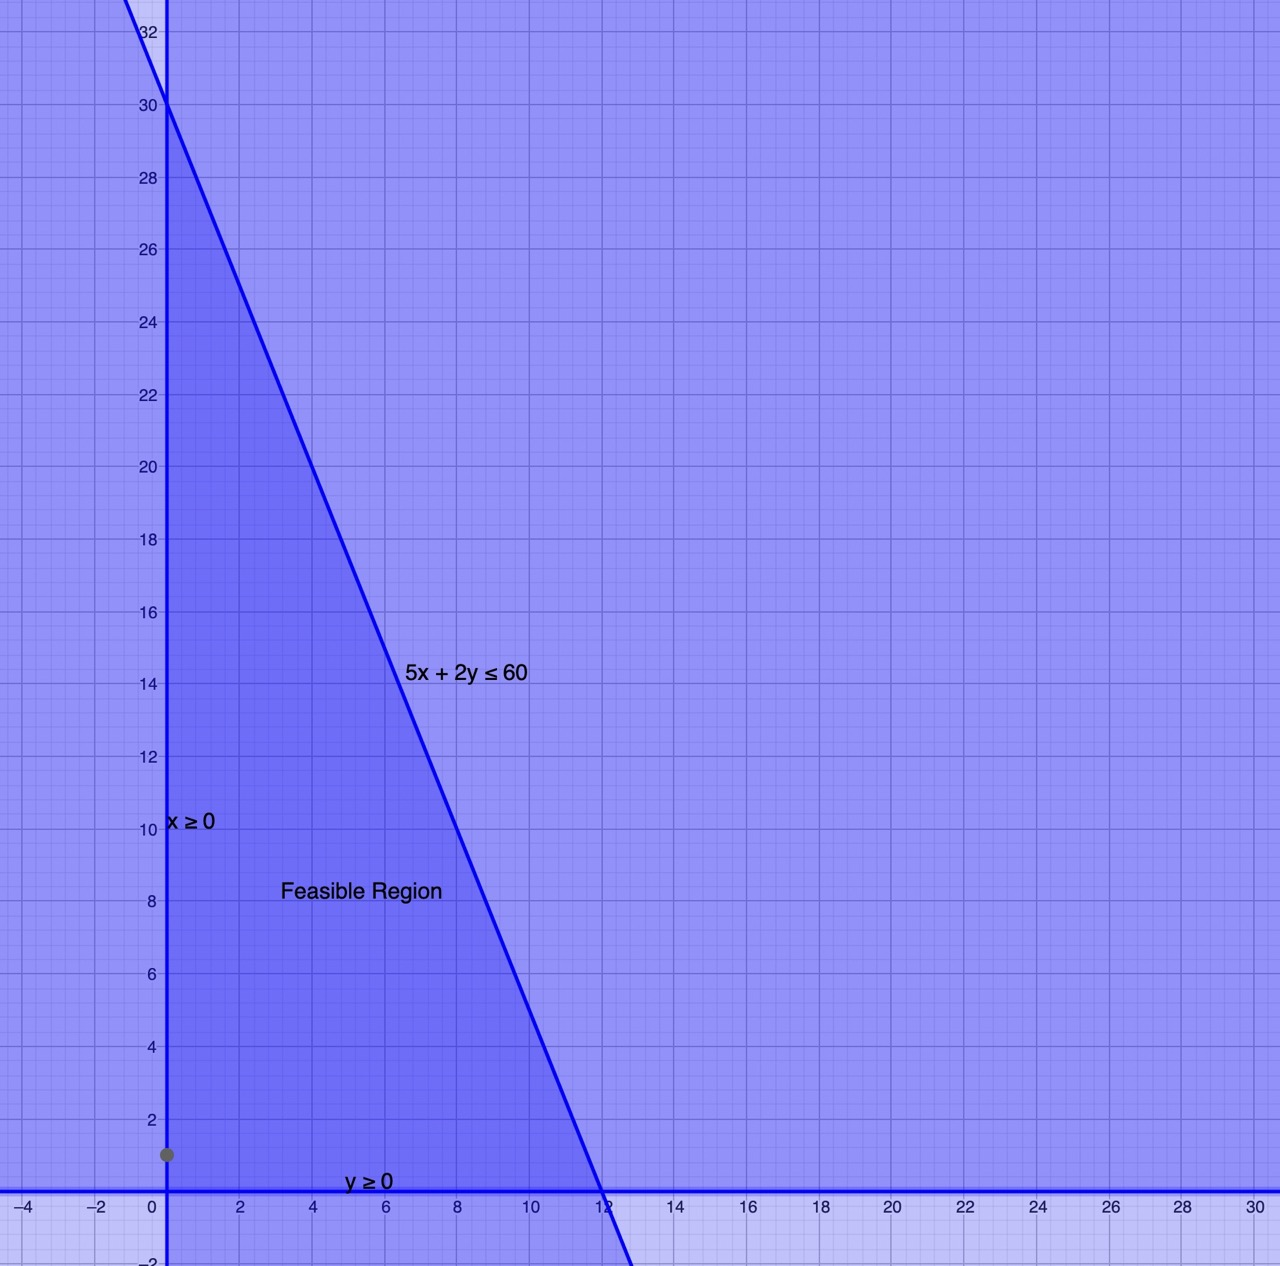
\includegraphics[width=0.8\textwidth,height=\textheight]{images/a.jpeg}

}

\caption{Graph of the Feasible Region}

\end{figure}

All points within the region labelled ``feasible region'' are possible
solution to our problem in the sense that they do not violate the
constraints. For example, if we take the point \((8,4\) as the solution,
the company would need to manufacture 8 skateboards and 4 dolls We can
use the profit function to compute the profit associated with this
choice as follows:

\begin{align}
P&=x+0.55y\\
&=8+(0.55\times 4)\\
&=\$10.20
\end{align}

Although this solution does not violate the constraints, it is easy to
show that there is another point that would yield a higher profit while
still obeying the constraints. Take, for example, the point \((2,14)\)
which means 2 skateboards and 20 dolls. The profit for this choice would
be higher. See below:

\begin{align}
P&=1.00 x+0.55y\\
&=2+(0.55\times 20)\\
&=\$13.0
\end{align}

Choosing the point in the feasible region that would result in maximum
profit (optimal production policy) is not a trivial task. However, there
is an genius technique known as \textbf{\emph{The Corner Point
Principle}} which we discuss next:

\hypertarget{the-corner-point-principle}{%
\subsection{The Corner Point
Principle}\label{the-corner-point-principle}}

The corner point principle has been touted as one of the most important
insights into the theory of linear programming. The principle states
that,

\begin{Shaded}
\begin{Highlighting}[]
\DataTypeTok{In} \DataTypeTok{a} \DataTypeTok{linear} \DataTypeTok{programming} \DataTypeTok{problem}\ErrorTok{,} \DataTypeTok{the} \DataTypeTok{maximum} \DataTypeTok{value} \DataTypeTok{for} \DataTypeTok{the} \DataTypeTok{profit} \DataTypeTok{formula} \DataTypeTok{always}
\DataTypeTok{corresponds} \DataTypeTok{to} \DataTypeTok{a} \DataTypeTok{corner} \DataTypeTok{point} \DataTypeTok{of} \DataTypeTok{the} \DataTypeTok{feasible} \DataTypeTok{region}\KeywordTok{.}
\end{Highlighting}
\end{Shaded}

For our linear programming problem above, there are three corners with
cor=ordinates \((0,0)\), \((0,30\), and \((12,0)\). So, we can compute
the profit associated with these 3 points and choose the highest as our
optimal production policy:

For \((0,0)\), the profit would be \(\$0\).

For \((0,30\), the profit would be, \(P=1.00 (0)x+0.55(30)=\$16.5\)

For \((12,0\), the profit would be, \(P=1.00 (12)x+0.55(0)=\$12.00\)

Therefore, the \textbf{\emph{optimal production policy}} would be to
manufacture 0 skateboards and 30 dolls.

\textbf{NOTE}: In the real world, there would be a lot more corners
which would make this process cumbersome. However, as you may have
guessed, there are computer programs that can do the job faster and more
efficiently than humans.

\hypertarget{summary-of-the-geometric-method}{%
\subsection{Summary of the Geometric
Method}\label{summary-of-the-geometric-method}}

\begin{enumerate}
\def\labelenumi{\arabic{enumi}.}
\tightlist
\item
  Read the problem carefully to identify resources and products.
\item
  Make a mixture chart for the problem.
\item
  Assign an unknown quantities (often \(x\), and \(y\)) to each product
  and use the mixture chart to write the resource and minimum
  constraints.
\item
  Write the profit formula as well.
\item
  Create a feasible region by graphing ther inequalities (you can use a
  program such as Geogebra or Desmos).
\item
  Find the coordinates of the corner points and evaluate the profit for
  each. The corner that gives maximum profit is the optimal production
  policy.
\end{enumerate}

In the next example, we extend the toy problem above to include one more
resource (person minutes). Read below:

\textbf{Example 2}

A toy manufacturer can manufacture only skateboards and, only dolls, or
some kind of skateboards and dolls. Skateboards require 5 units of
plastic and can be sold for a profit of \$ 1, while dolls require 2
units of plastic and can be sold for \$0.55 profit. Only 60 units of
plastic are available. Furthermore, making one skateboard requires 15
person-minutes while making one doll requires 18-person minutes. There
are only 360person person-minutes available.

\begin{enumerate}
\def\labelenumi{(\alph{enumi})}
\tightlist
\item
  Make a mixture chart to model this situation.
\item
  What numbers of skateboards and/or dolls should the company make to
  maximize profit?
\end{enumerate}

\textbf{\emph{Solution}}

\begin{enumerate}
\def\labelenumi{\alph{enumi})}
\tightlist
\item
  Below is the new mixture chart,
\end{enumerate}

\begin{longtable}[]{@{}
  >{\centering\arraybackslash}p{(\columnwidth - 6\tabcolsep) * \real{0.2917}}
  >{\centering\arraybackslash}p{(\columnwidth - 6\tabcolsep) * \real{0.2361}}
  >{\centering\arraybackslash}p{(\columnwidth - 6\tabcolsep) * \real{0.2361}}
  >{\raggedleft\arraybackslash}p{(\columnwidth - 6\tabcolsep) * \real{0.2361}}@{}}
\toprule\noalign{}
\begin{minipage}[b]{\linewidth}\centering
Products
\end{minipage} & \begin{minipage}[b]{\linewidth}\centering
Resource 1: Plastic: 60
\end{minipage} & \begin{minipage}[b]{\linewidth}\centering
Resource 2: person-minutes 360
\end{minipage} & \begin{minipage}[b]{\linewidth}\raggedleft
Profit
\end{minipage} \\
\midrule\noalign{}
\endhead
\bottomrule\noalign{}
\endlastfoot
Skateboard (x units) & 5 & 15 & \$ 1.00 \\
Dolls(y units) & 2 & 18 & \$ 0.55 \\
\end{longtable}

\begin{enumerate}
\def\labelenumi{\alph{enumi})}
\setcounter{enumi}{1}
\tightlist
\item
  We start by writing down the inequalities (constraints) and the profit
  function. We still have the same minimum constraints as from example
  1: \[x \ge 0 \hspace{.04in} \text{and} \hspace{.04in} y \ge 0\] For
  the resource constraints, we have two inequalities because we have two
  resources: For the plastic, we have \[5x+2y\le60\] For the person
  hours, we have, \[15x + 18y \le 360\] The profit function stays the
  same: \[P=1x+0.55y\] Next, we create a feasible region by graphing the
  inequalities. Notice that this new feasible region is smaller than the
  first and it has four corner points. The fourth point is as a result
  of the new inequality created by the additional resource constraints.
  As indicated earlier, the more resources you have, the more the corner
  points you expect.
\end{enumerate}

\begin{figure}

{\centering 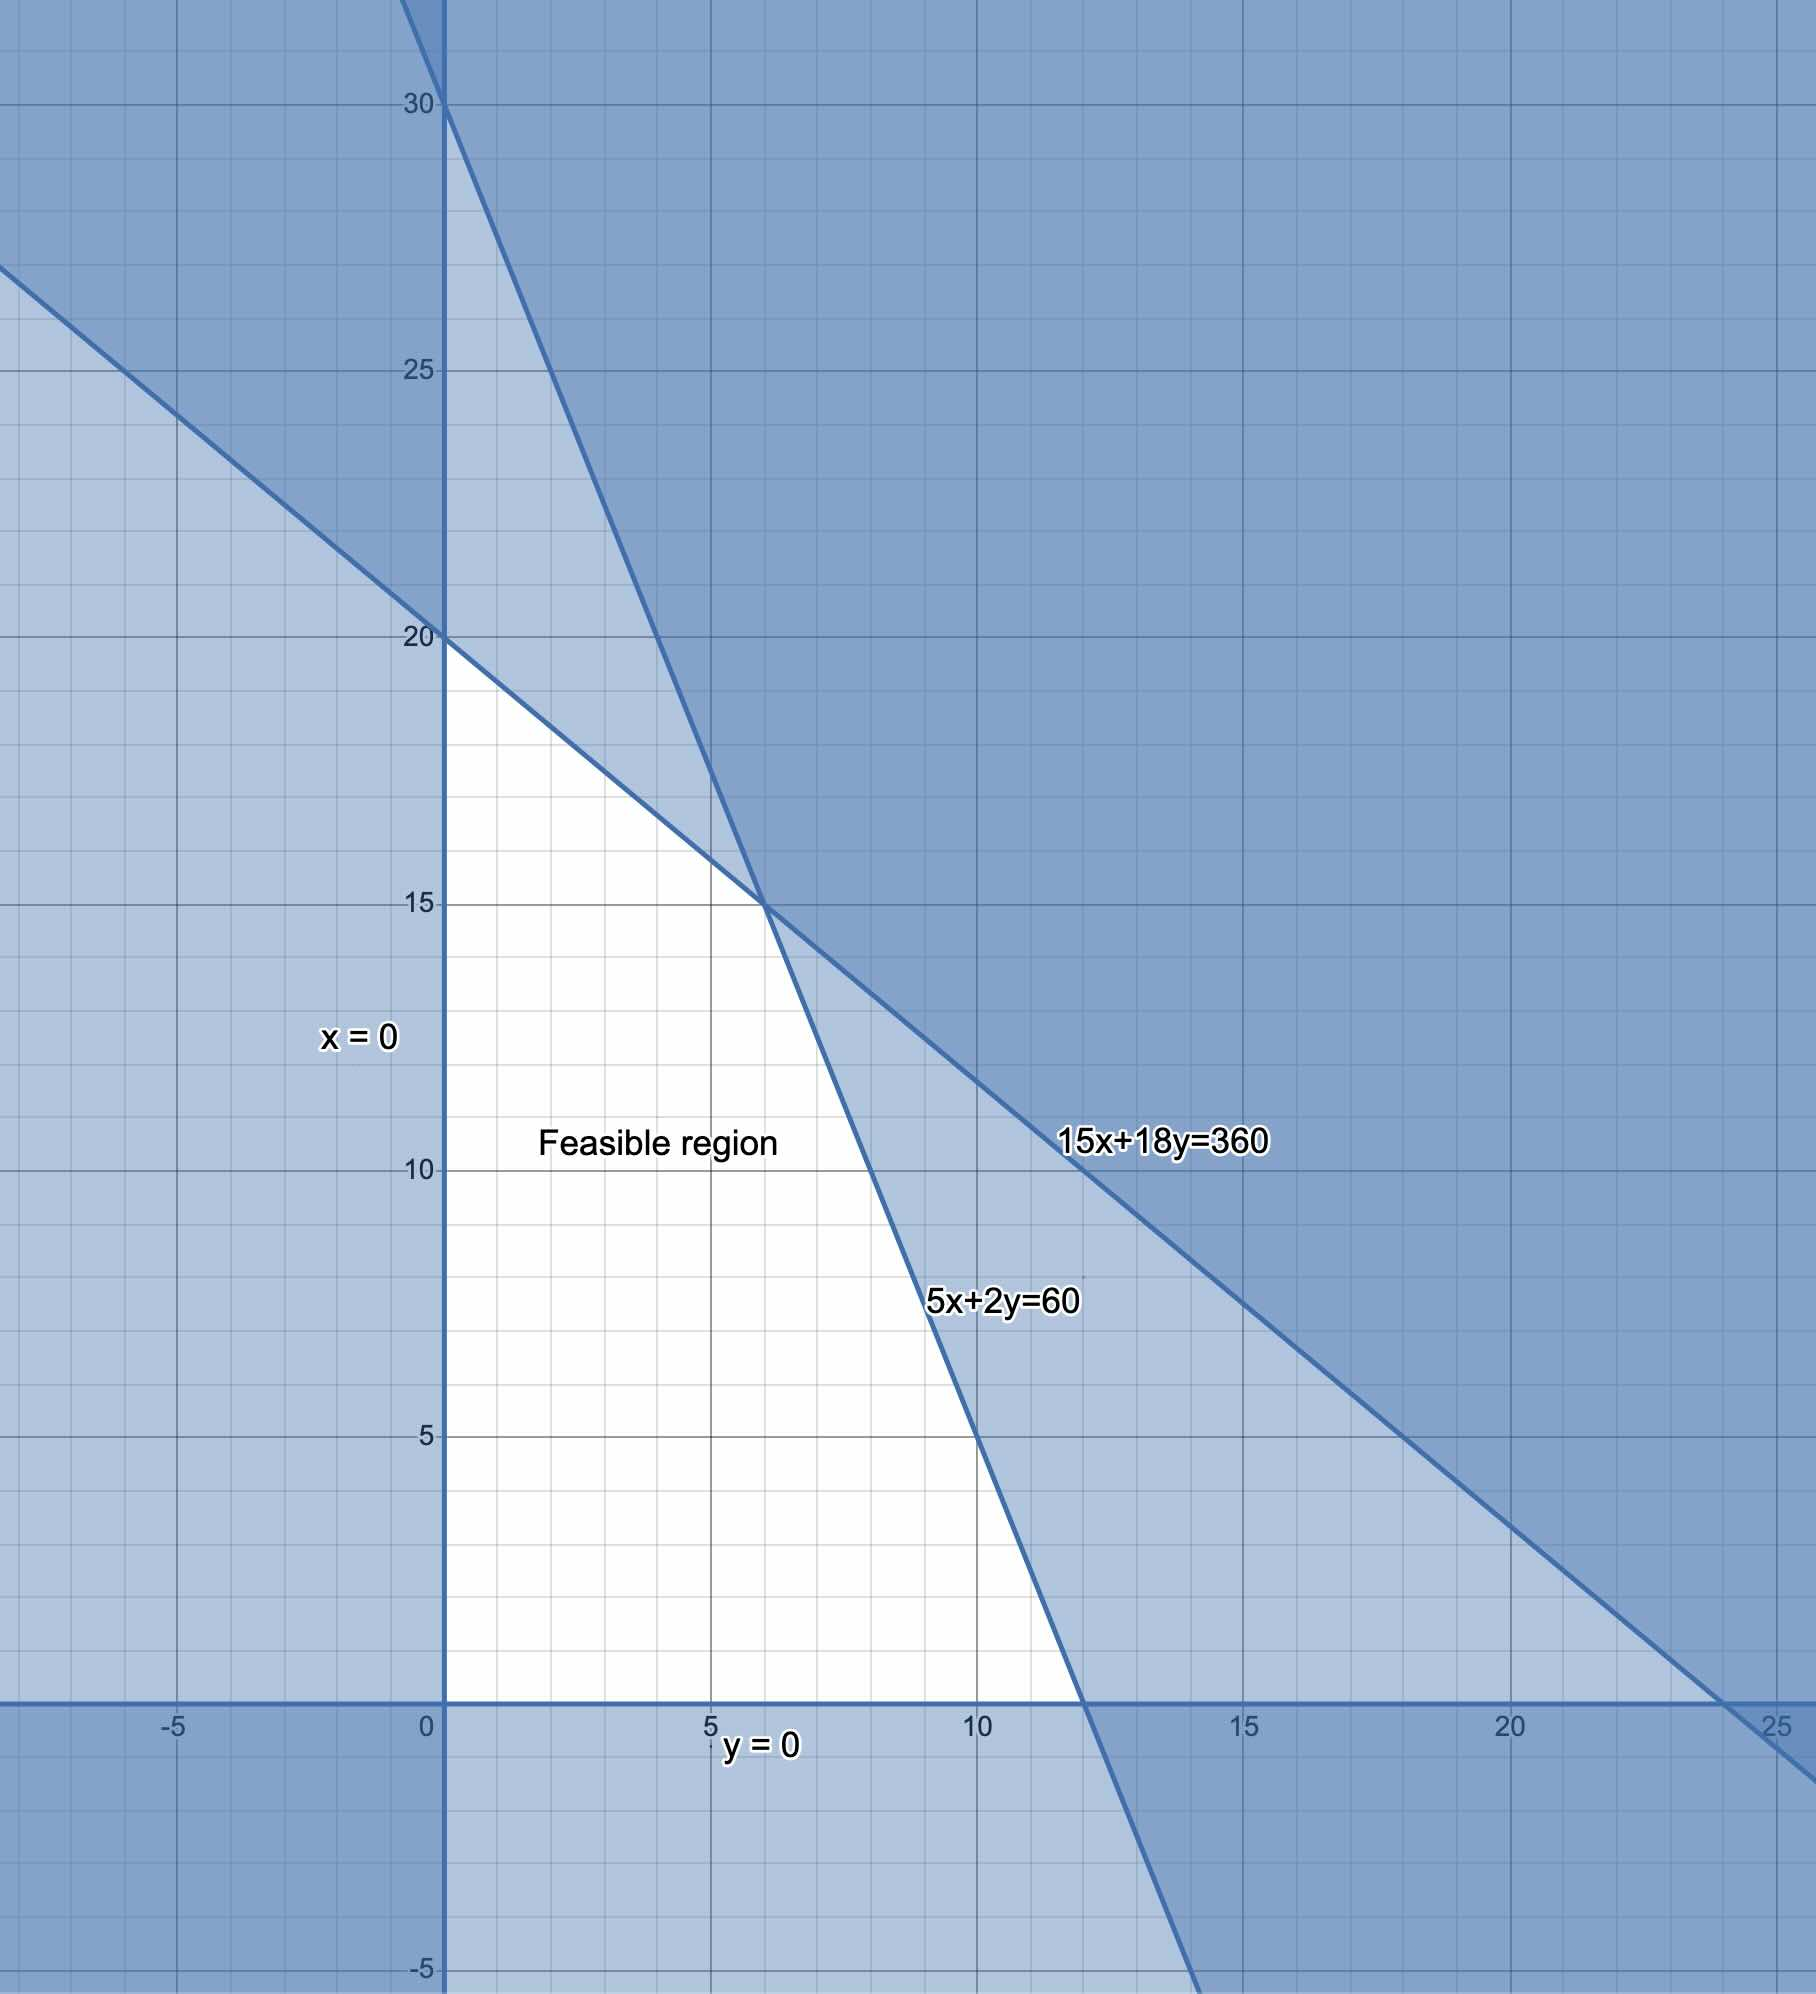
\includegraphics[width=0.8\textwidth,height=\textheight]{images/b.jpeg}

}

\caption{Updated Feasible Region}

\end{figure}

The last step is to use the corner principle to find the optimal
production policy: We check the profits for each of the corner:

For \((0,0)\), the profit would be \(\$0\).

For \((0,20\), the profit would be, \(P=1.00 (0)x+0.55(20)=\$11.00\)

For \((6,15\), the profit would be, \(P=1.00 (6)x+0.55(15)=\$14.50\)

For \((12,0\), the profit would be, \(P=1.00 (12)x+0.55(0)=\$12.00\)

Thus, in this new problem, the optimal production policy is 6
skateboards and 15 dolls for a maximum profit of \$ 14.50.

\hypertarget{section-exercises}{%
\subsection{Section Exercises}\label{section-exercises}}

For each description in exercises 1-4,create a mixture table and write
one or more resource constraint inequalities. The unknown to use for
each product is given in parenthesis:

\begin{enumerate}
\def\labelenumi{\arabic{enumi}.}
\tightlist
\item
  Manufacturing one package of hot dogs(x) requires 6 oz of beef, and
  manufacturing one package of bologna (y) requires 4 oz of beef. There
  are 300 oz of beef available.
\item
  It takes 30 ft of 12-in. board to make one bookcase (x); it takes 72
  ft of 12-in. board to make one table(y). There are 420 ft of 12-in.
  board available.
\item
  Manufacturing one salami(x) requires 12 oz of beef and 4 oz of pork.
  Manufacturing one bologna (y) requires 10 oz of beef and 3 oz of pork.
  There are 40 lb of beef and 480 oz of pork available.
\end{enumerate}

For each of the following exercises, graph the feasible region, label
each line segment bounding it with appropriate equation, and give the
coordinates of every corner point.

\begin{enumerate}
\def\labelenumi{\arabic{enumi}.}
\setcounter{enumi}{3}
\item
  \(x\ge 0\) ; \(y\ge 0\); \(2x+y\le10\)
\item
  \(x\ge 0\) ; \(y\ge 0\); \(x+2y\le12\); \(x+2y\le8\)
\item
  \(x\ge 2\) ; \(y\ge 6\); \(3x+2y\le30\)
\item
  Determine whether the points \((2,4)\) and/or \((10,6)\) are points of
  the feasible region in exercises 4, 5, and 6.
\item
  Determine the maximum value of \(P\) given by \(P=3x+2y\) subject to
  the constraints \(x\ge 0\), \(y\ge 0\), \(x\le 7\), and \(y\le 5\).
\item
  A linear programming problem has the following constraints: \(x\ge0\),
  \(y\ge0\), \(5x-y\le15\), and \(4y+x\le24\).

  \begin{enumerate}
  \def\labelenumii{\alph{enumii})}
  \tightlist
  \item
    Without graphing, determine the corner points of the feasible region
    for the LP problem?
  \item
    Sketch a graph of the feasible region.
  \end{enumerate}
\item
  Nuts Galore sells two spiced nut mixtures: Grade A and Grade B. Grade
  A requires 7 oz of peanuts and for every 8 oz of almonds. Grade B
  requires 9 oz of peanuts for every 8 oz of almonds. There are 630 oz
  of peanuts 640 oz of almonds available. Grade A makes Nuts Galore a
  profit of \$1.70, and Grade B makes a profit of \$2.40 per unit
  assembled. How many units of Grade A and Grade B nut mixtures should
  be made to maximize the company's profit, assuming that all the units
  can be sold?
\item
  Find the maximum value of \(P\) where \(P=3x+2y\) subject to the
  constraints \(x\ge3\), \(y\ge2\), \(x+y\le10\), and \(2x+3y\le24\).
\item
  A clothing manufacturer has 600 yd of cloth available to make shirts
  and decorated vests. Each shirt requires 3 yd of material and provides
  a profit of \$5. Each vest requires 2 yd of material and provides a
  profit of \$2. The manufacturer wants to guarantee that under all
  circumstances, there are minimums of 100 shirts and 30 vests produced.
  How many of each garment should be made to maximize the profit? If
  there are no minimum quantities, how, if at all, does the optimal
  production policy change?
\item
  A paper recycling company uses scrap cloth and scrap paper to make two
  different grades of recycled paper. A single batch of grade A recycled
  paper is made from 25 lb of scrap cloth and 10 lb of scrap paper,
  whereas one batch of grade B recycled paper is made from 10 lb of
  scrap cloth and 20 lb of scrap paper. The company has 100 lb of scrap
  cloth and 120 lb of scrap paper on hand. A batch of grade A paper
  brings a profit of \$500, whereas a batch of grade B paper brings a
  profit of \$250. What amounts of each grade should be made? How, if at
  all, do the maximum profit and optimal production policy change if the
  company is required to produce at least one batch of each type?
\item
  Courtesy Calls makes telephone calls for businesses and charities. A
  profit of \$0.50 is made for each business calls and \$0.40 for each
  charity call.It takes 4 min (on average) to make a business call and 6
  min (on average) to make a charity call. If there are 240 min of
  calling time to be distributed each day, how should that time be spent
  so that Courtesy Calls makes a maximum profit? What changes, if any,
  occur in the maximum profit and optimal production policy if they must
  make at least 12 business calls and 10 charity call every day?
\end{enumerate}

\hypertarget{the-simplex-method}{%
\section{The Simplex Method}\label{the-simplex-method}}

Before we introduce the

\hypertarget{the-transportation-problem}{%
\section{The Transportation Problem}\label{the-transportation-problem}}

\hypertarget{the-simplex-method-1}{%
\chapter{The Simplex Method}\label{the-simplex-method-1}}

\hypertarget{introduction-to-simplex-method}{%
\section{Introduction to Simplex
Method}\label{introduction-to-simplex-method}}

As stated earlier, Linear Programming is one of the most commonly used
methods for solving practical problems in business and even in
government. However, the problems we have considered so far had a
maximum of two products and relatively small feasible regions and few
corner points. Many real life problems often involve much more products
and result in very big feasible regions with hundreds or even thousands
of corner points.

As an example, consider the following LP problem:

\textbf{Example 1}

A factory manufactures chairs, tables and bookcases each requiring the
use of three operations: Cutting, Assembly, and Finishing. The first
operation can be used at most 600 hours; the second at most 500 hours;
and the third at most 300 hours. A chair requires 1 hour of cutting, 1
hour of assembly, and 1 hour of finishing; a table needs 1 hour of
cutting, 2 hours of assembly, and 1 hour of finishing; and a bookcase
requires 3 hours of cutting, 1 hour of assembly, and 1 hour of
finishing. If the profit is \$20 per unit for a chair, \$30 for a table,
and \$25 for a bookcase, how many units of each should be manufactured
to maximize profit?

Let us start by creating a mixture chart for the problem:

\begin{longtable}[]{@{}
  >{\raggedright\arraybackslash}p{(\columnwidth - 8\tabcolsep) * \real{0.1494}}
  >{\centering\arraybackslash}p{(\columnwidth - 8\tabcolsep) * \real{0.2069}}
  >{\centering\arraybackslash}p{(\columnwidth - 8\tabcolsep) * \real{0.2184}}
  >{\centering\arraybackslash}p{(\columnwidth - 8\tabcolsep) * \real{0.2299}}
  >{\centering\arraybackslash}p{(\columnwidth - 8\tabcolsep) * \real{0.1609}}@{}}
\toprule\noalign{}
\begin{minipage}[b]{\linewidth}\raggedright
Products
\end{minipage} & \begin{minipage}[b]{\linewidth}\centering
Resource:

Cutting(600hrs)
\end{minipage} & \begin{minipage}[b]{\linewidth}\centering
Resource:

Assembly(500hrs)
\end{minipage} & \begin{minipage}[b]{\linewidth}\centering
Resource:

Finishing(300hrs)
\end{minipage} & \begin{minipage}[b]{\linewidth}\centering
Profit (\$)
\end{minipage} \\
\midrule\noalign{}
\endhead
\bottomrule\noalign{}
\endlastfoot
Chairs & 1 & 1 & 1 & 20 \\
Tables & 1 & 2 & 1 & 30 \\
Bookcases & 3 & 1 & 1 & 25 \\
\end{longtable}

Next, we make the constraint inequalities assuming that the company
makes \(x\) chairs, \(y\) tables, and \(z\) bookcases. Note that using
\(x,y\), and \(z\) is not advisable when you have more than 3 variables.
It is recommended you use \(x_1, x_2, x_3,...\)

\textbf{Minimum constraints:} Chairs: \(x\ge 0\) Tables: \(y\ge 0\)
Bookcases: \(z\ge 0\).

\textbf{Resource constraints:} For cutting: \(x+y+3z\le600\) For
assembly: \(x+2y+z\le500\) For finishing: \(x+y+z\le300\)

\textbf{Things to Note}

\begin{itemize}
\tightlist
\item
  Unlike the problems encountered in the previous chapter, this problem
  includes 3 variables \((x,y, z).\) This means that, we would have to
  create a three dimensional graph to visualize the feasible region- a
  task that is impossible for humans to execute by hand.
\item
  Most application problems include way more than 3 variables, which
  means we would need a multidimensional graph to visualize the feasible
  region.
\item
  The simplex method provides an algorithmic method that solves this
  type of problems without needing to create a visual feasible region.
  The method can also be used to solve problems in the previous chapter.
\item
  The technical details of the simplex method are beyond the scope of
  the course but the algorithm itself is relatively easy to execute once
  you learn it.
\end{itemize}

We will return to this problem later.

\hypertarget{step-by-step-simplex-method}{%
\section{Step-by-Step Simplex
Method}\label{step-by-step-simplex-method}}

We want to walk through the simplex method step-by-step until we find an
optimal production policy and the maximum profit.

Consider the example below:

\textbf{Example 2}

Maximize the function \(P=3x+4y+z\) subject to the conditions

\[3x+10y+5z \le 120 \] \[5x+2y+8z \le 6\] \[8x+10y+3z \le 105\]

\textbf{\emph{Problem Posing:}} Note that this problem does not have a
real world context, before you proceed, please write a real life LP
problem that might suit the given profit function and constraints.

\textbf{Step 1:} Convert the inequalities to equations by adding
\textbf{slack variables} and rewrite the profit function so that the
constant value is on the right hand side of the equation:
\[3x+10y+5z+s_1 = 120 \] \[5x+2y+8z +s_2= 6\] \[8x+10y+3z +s_3= 105\]
\[-3x-4y-z+P\] Slacks allow us to convert inequalities to equations by
filling up the amount by which a quantity falls short of another. For
example, \(s_1\) is the amount by which the quantity \(3x+10y+5z\) falls
short of 120. So, by adding \(s_1\) to \(3x+10y+5z\) we achieve the
equality. sh

\textbf{Step 2:} Create the initial \textbf{simplex tableau}. In the
tableu, each equation appears in its own row with the profit function
appearing as the last row. See table below:

\begin{figure}

{\centering 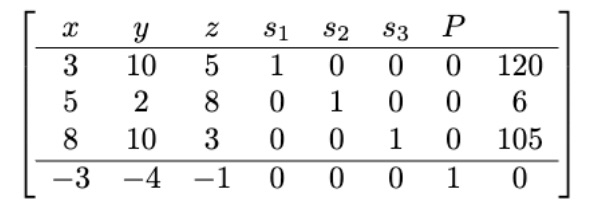
\includegraphics[width=0.5\textwidth,height=\textheight]{images/c.jpeg}

}

\caption{Initial Tableau}

\end{figure}

\textbf{Step 3:} Choose the pivot column. The most negative entry in the
last row is -4 which is in column 2. So, column 2 is our pivot column.
See below:

\begin{figure}

{\centering 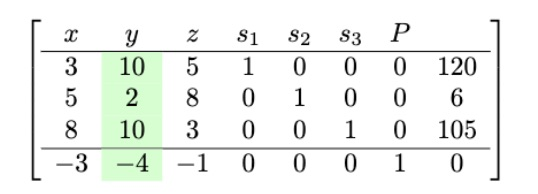
\includegraphics[width=0.5\textwidth,height=\textheight]{images/d.jpeg}

}

\caption{Tableau showing Pivot column}

\end{figure}

Why do we choose the most negative element in the last row?

The most negative entry in the bottom row represents the largest
coefficient in the objective function - the coefficient whose entry will
increase the value of the objective function the quickest. Remember this
is a maximization problem.

\textbf{Step 4:} Find the pivot row. To find the pivot row, divide the
values on the far right by values of the pivot column. The row with the
smallest quotient will be your pivot row. In this case, \[120/10=12\]
\[6/2=3\] \[105/110=10.5\] The smallest quotient here is 3, which means
the pivot row is row 2. The matrix below highlight the picot row:

\begin{figure}

{\centering 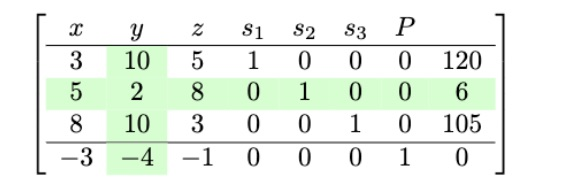
\includegraphics[width=0.5\textwidth,height=\textheight]{images/e.jpeg}

}

\caption{Pivot row and column}

\end{figure}

Why does the smallest quotient identify a row? Using the quotients to
identify the pivot element guarantees that we do not violate the
constraints as we proceed with the algorithm.

\textbf{Step 5:} The 2 at the intersection of row 2 and column 2 is
called a pivot element. We want to perform row operations to make it a
1. To do this, we simply divide the whole of row 2 by 2. This can be
represented as \(\frac{1}{2}R_2 \mapsto R_2\). This means that the new
row 2 will be half of the previous row 2.

\(\frac{1}{2}\times(5,2,8,0,1,0,0,6)=(2.5,1,4,0,.5,0,0,3)\)

The new tableau becomes,

\begin{figure}

{\centering 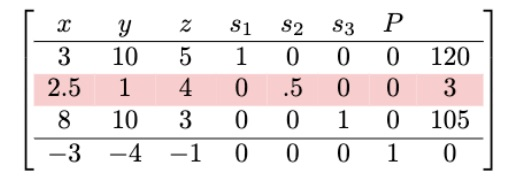
\includegraphics[width=0.5\textwidth,height=\textheight]{images/f.jpeg}

}

\caption{Unitize pivot element}

\end{figure}

\textbf{Step 6:} We perform row operations to convert every entry above
and below the new pivot element (1) into a 0. The following operations
will achieve this:

\begin{itemize}
\tightlist
\item
  The new row 1 will be the difference between row and and 10 times row
  2 i.e., \(R_1 - 10R_2\mapsto R_1\).
\item
  The new row 3 will be the difference between the current row 3 and 10
  times row 2.e., \(R_3 - 10R_2\mapsto R_3\).
\item
  The new row 4 will be the current row 4 plus 4 times row 2 i.e.,
  \(R_4 + 4R_2\mapsto R_4\).
\end{itemize}

We perform the actual computations below:

\(R_1 - 10R_2\mapsto R_1\):
\((3,10,5,1,0,0,0,120) - 10(2.5,1,4,0,0.5,0,0,3)=(-22,0,-35,1,-5,0,0,90)\).

\(R_3 - 10R_2\mapsto R_3\):
\((8,10,3,0,0,1,0,105) - 10(2.5,1,4,0,0.5,0,0,3)=(17,0,-37,0,-5,1,0,75)\).

\(R_4 + 4R_2\mapsto R_4\):
\((-3,-4,-1,0,0,0,1,0) + 4(2.5,1,4,0,0.5,0,0,3)=(7,0,15,0,2,0,1,12)\).

Now we put these new rows into our tableau. See below:

\begin{figure}

{\centering 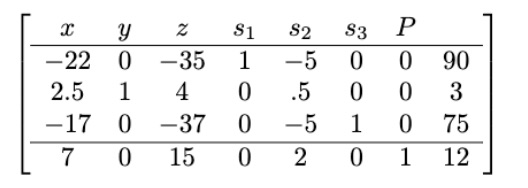
\includegraphics[width=0.5\textwidth,height=\textheight]{images/g.jpeg}

}

\caption{One more Tableau}

\end{figure}

\textbf{Notice that} the last row has no negative numbers. This means we
are done and we can directly read our solution. If there were any
negative numbers left on the last row, you would have to do the process
one more time (i.e., find new pivot column and row then perform
subsequent row operations). This process continues until there are no
negative numbers on the last row.

\textbf{Step 7:} Read the solution from the final tableau. Every column
with a ``1's'' and ``0's'' would give us a value for a variable. In our
case above,

\(y=3, s_1=90, s_3=75, P=12\)

Al the others (i.e., \((x,z,s_2)\)) will be zero.

This solution basically means, make 3 units of product \(y\), and zero
product \(x\) and \(z\).

\hypertarget{the-transportation-problem-1}{%
\chapter{The Transportation
Problem}\label{the-transportation-problem-1}}

\part{Mathematics of Finance}

\hypertarget{simple-interest}{%
\chapter{Simple Interest}\label{simple-interest}}

\hypertarget{compound-interest}{%
\chapter{Compound Interest}\label{compound-interest}}

\hypertarget{annuities-and-sinking-funds}{%
\chapter{Annuities and Sinking
Funds}\label{annuities-and-sinking-funds}}

\bookmarksetup{startatroot}

\hypertarget{summary}{%
\chapter{Summary}\label{summary}}

In summary, this book has no content whatsoever.

\begin{Shaded}
\begin{Highlighting}[]
\DecValTok{1} \SpecialCharTok{+} \DecValTok{1}
\end{Highlighting}
\end{Shaded}

\begin{verbatim}
[1] 2
\end{verbatim}

\bookmarksetup{startatroot}

\hypertarget{references}{%
\chapter*{References}\label{references}}
\addcontentsline{toc}{chapter}{References}

\markboth{References}{References}

\hypertarget{refs}{}
\begin{CSLReferences}{1}{0}
\leavevmode\vadjust pre{\hypertarget{ref-knuth84}{}}%
Knuth, Donald E. 1984. {``Literate Programming.''} \emph{Comput. J.} 27
(2): 97--111. \url{https://doi.org/10.1093/comjnl/27.2.97}.

\end{CSLReferences}



\end{document}
